\documentclass[14pt]{extarticle}
\usepackage[
left=25mm,
top=20mm,
right=15mm,
bottom=20mm,
]{geometry}

%\usepackage{graphicx}
\usepackage[pdftex]{graphicx}
\usepackage[utf8x]{inputenc}
\usepackage[russian]{babel}
\usepackage[T1]{fontenc}
\usepackage{float}
\usepackage{listings}
\usepackage{cite}
\usepackage{hyperref}
\usepackage{etoolbox}
\usepackage{indentfirst}
\usepackage[linesnumbered,boxed]{algorithm2e}
%\sloppy

\lstset{
	sensitive=true,
	basicstyle=\small,
	keywordstyle=\color{black},
	commentstyle=\scriptsize\rmfamily,
	keywordstyle=\ttfamily\underbar,
	identifierstyle=\ttfamily,
	basewidth={0.5em,0.5em},
	columns=fixed,
	fontadjust=true,
	literate={->}{{$\to$}}1
}

\makeatletter
%\renewcommand{\@biblabel}[1]{#1.} % Заменяем библиографию с квадратных скобок на точку:
\makeatother
\gappto\captionsrussian{\renewcommand{\contentsname}{Оглавление}}
\renewcommand\baselinestretch{1.5}
\renewcommand{\lstlistingname}{Листинг}

\begin{document}
	
	\begin{titlepage}
		\thispagestyle{empty}
		\def\baselinestretch{1.0}
		\begin{center}
			{САНКТ-ПЕТЕРБУРГСКИЙ ГОСУДАРСТВЕННЫЙ УНИВЕРСИТЕТ \\ \vskip 0.3em {\large Математико-механический факультет \\ \vskip 0.7em{\large Кафедра системного программирования \\}}}
			\vspace*{0.15\textheight}
			{\large Гудиев Артур Владимирович}
			
			\vskip 2em
			{\LARGE Реализация примитвов и оконного менеджера для построения пользователских интерфейсов на языке PostScript}
			
			\vskip 1em
			{\large Дипломная работа} \\
			\vskip 2em
			{\normalsize \raggedleft 
				Допущена к защите.\\
				Зав. кафедрой:\\
				д.ф.-м.н., проф. А.Н. Терехов
				\\[2em]
				Научный руководитель:\\
				к.ф.-м.н. Д.Ю. Булычев
				\\[2em]
				Рецензент:\\
				Д.В. Кознов
				\\[2em]
				%Неизвестно \\
				\vspace*{0.08\textheight}
				{\centering Санкт-Петербург \\ 2015}
			}
		\end{center}
	\end{titlepage}
	\begin{titlepage}
		\thispagestyle{empty}
		\def\baselinestretch{1.0}
		\begin{center}
			{SAINT-PETERSBURG STATE UNIVERSITY \\ \vskip 0.3em {\large Mathematics \& Mechanics Faculty \\ \vskip 0.7em{\large Department of Software Engineering \\}}}
			\vspace*{0.15\textheight}
			{\large Artur Gudiev}
			
			\vskip 2em
			{\LARGE Window manager and GUI primitives for user interface implementation in PostScript}
			
			\vskip 1em
			{\large Graduation Thesis} \\
			\vskip 2em
			{\normalsize \raggedleft 
				Adnitted for defence.\\
				Head of the chair:\\
				professor  Andrey Terekhov
				\\[3em]
				Scientific supervisor:\\
				Dmitri Boulytchev
				\\[3em]
				Reviewer:\\
				Dmitri Koznov
				\\[2em]
				%Неизвестно \\
				\vspace*{0.08\textheight}
				{\centering Saint-Petersburg \\ 2015}
			}
		\end{center}
	\end{titlepage}
	
	\tableofcontents
	\thispagestyle{empty} 
	\pagebreak
	
	
	
	\section*{Введение}
	\addcontentsline{toc}{section}{Введение}
	Язык PostScript - это графический интерпретируемый язык программирования, создавашийся с целью представления графики в машинонезависимой форме. Посредством графических операторов языка PostScript можно отобразить на экране прямые и кривые линии, залить цветом область, определить область рисования, задать графические параметры.  
	
	Графический интерфейс пользователя - это разновидность пользовательского интерфейса, в котором элементы интерфейса представлены в виде графических примитивов. Визуальные интерфейсы пользователя упрощают работу с программами, делая ее наглядной. Язык PostScript обладает базовыми графическими возможностями для отображения внешнего вида графических интерфейсов.
	
	Оконный менеджер — это приложение, управляющее размещением окон и определяющая их внешний вид в оконной системе графического интерфейса. Оконные менеджеры работают на основе существующей оконной системы. Кроме того оконный менеджер включает в себя и визуальные эффекты, проявляющиеся во время работы с окнами. Обычно оконный менеджер привязан к конкретной операционной системе. Язык PostScript позволяет нарисовать такие объекты, как элементы графического интерфейса пользователя и визуальные эффекты оконного менеджера.
	
	Ранее в рамках проекта лаборатории JetBrains был реализован интерпретатор графического языка PostScript, однако с его помощью было трудно создавать графические интерфейсы и оконный менеджер из-за того, что, например, в PostScript не поддерживается механизм обработки событий. Для упрощения реализации этой возможности планируется расширить язык PostScript. Данная работа ведется по трем направлениям: оптимизация интерпретатора (Д. Поздин), обработка событий (Р. Макулов) и реализация графических примитивов и оконного менеджера (А. Гудиев).
	
	Целью данной дипломной работы является реализация графических примитивов и оконного менеджера для создания пользовательских интерфейсов на языке PostScript.
	
	\pagebreak
	\section{Обзор}
	\subsection{ Описание существующих решений }
		\subsubsection{Qt Quick}
		\subsubsection{Java Swing}
		\subsubsection{ Недостатки существующих решений }
		
	\subsection{Описание используемых инструментов }
		\subsubsection{JVM}
		\subsubsection{Java Swing}
		\subsubsection{ Интерпретатор JB }
		Интерпретатор PostSc
		
	\subsection{ Проект рабочей группы интерпретатора PostScript }
Задача реализации интерпретатора графического языка PostScript решается в рамках проекта компании JetBrains. 
		
		Проект можно разделить на задачи:
		\begin{itemize}
		\item Оптимизация интерпретатора
		\item Реализация механизма обработки событий
		\item Реализация примитивов и оконного менеджера		
		\end{itemize}	
	
	\pagebreak
	\section{Примитивы графической библиотеки}
	\subsection{Структура графических примитивов}
		Есть файл графческой библиотеки - glib.ps. В нем создается словарь gelements. У каждого примитива есть свой номер, по которому он хранится в словаре gelements. 
		
		Общий предок у всех - объект сцена (scene). У каждого примитива есть дети-примитвы. Номера детей хранятся в поле-массиве children.
		
		Каждому графическому примитиву соответствуют два файла - файл с описанием объекта и файл с процедурой отрисовки примитива. (Например, для кнопки - это button.ps и paintButton.ps). 
		
		В файле первом есть два конструктора - абсолютный и относительный. У каждого примитива есть свои координаты и размеры. Если координаты задаются относительно родителя, то вызывается относительный контсркутор. Если примитив задается абсолютными координатами, тогда вызывается абсолютный. Например, пусть есть окно с левым нижним концом в точке (0,0), высотой 1000 и шириной 1000. Пусть от окна наследуется кнопка с левым нижним концом в (200, 300), длиной 400 и шириной 500. 
		
		Тогда при задании абсолютными координатами 		
		200 300 400 500 ... button
		
При задании относительными
		0.2 0.3 0.4 0.5	... relButton.
		
		
Относительные координаты хороши тем, что при изменении размеров или сдвиге родителя, они не изменяются.

На каждый примитив можно повесить событие - процедуру PostScript. Их может быть несколько. У каждого графического объекта есть словарь eventProcDict, в нем хранятся процедуры, которые вызываются при событии у объекта. 
	
	\subsection{Кнопка}
	ывфы
		\begin{figure}[h]
		\begin{center}
		\begin{minipage}[h]{0.4\linewidth}
		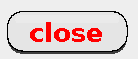
\includegraphics[width=180pt]{pictures/close1.png}
		\caption{ Кнопка} %% подпись к рисунку
		\label{ris:b1} %% метка рисунка для ссылки на него
		\end{minipage}
		\hfill 
		\begin{minipage}[h]{0.4\linewidth}
		
\includegraphics[width=180pt]{pictures/close2.png}
		\caption{Нажатая кнопка}
		\label{ris:b2}
		\end{minipage}
		\end{center}
		\end{figure}	
		
	\subsection{Флажок}
	Флажок - примитив, который содержит только два состояния.
		\begin{figure}[h]
		\begin{center}
		\begin{minipage}[h]{0.4\linewidth}
		
\includegraphics[width=180pt]{pictures/checkBox1.png}
		\caption{Флажок} %% подпись к рисунку
		\label{ris:b1} %% метка рисунка для ссылки на него
		\end{minipage}
		\hfill 
		\begin{minipage}[h]{0.4\linewidth}
		
\includegraphics[width=180pt]{pictures/checkBox2.png}
		\caption{Отмеченный флажок}
		\label{ris:b2}
		\end{minipage}
		\end{center}
		\end{figure}	
			
	Флажок важен для интерфейсов.	
		
	\pagebreak		
	\subsection{Поле со списком}
	Поле со списком предоставляет пользователю варианты.
	
		\begin{figure}[h]
		\begin{center}
		\begin{minipage}[h]{0.4\linewidth}
		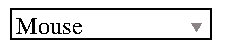
\includegraphics[width=180pt]{pictures/comboBox1.png}
		\caption{ Поле со списком} %% подпись к рисунку
		\label{ris:b1} %% метка рисунка для ссылки на него
		\end{minipage}
		\hfill 
		\begin{minipage}[h]{0.4\linewidth}
		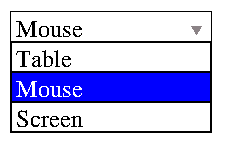
\includegraphics[width=180pt]{pictures/comboBox2.png}
		\caption{Раскрытое поле со списком}
		\label{ris:b2}
		\end{minipage}
		\end{center}
		\end{figure}
		
	\subsection{Список}
	Список - примитив с вариантами.
		\begin{figure}[h]
		\center{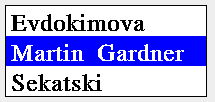
\includegraphics[width=180pt]{pictures/listBox.png}}
		\caption{Список}
		\label{ris:image}
		\end{figure}	
	
	\subsection{Метка}
		Метка - это текст по сути.
		\begin{figure}[h]
		\center{
\includegraphics[width=180pt]{pictures/label.png}}
		\caption{ Метка }
		\label{ris:image}
		\end{figure}	

	\subsection{Поле редактирования}
		Поле редактирования - это место, куда печатается текст.
		\begin{figure}[h]
		\center{
\includegraphics[width=180pt]{pictures/textField.png}}
		\caption{ Поле редактирования }
		\label{ris:image}
		\end{figure}	
	\subsection{Радиокнопка}
		Кнопка, два варианта включения.
		\begin{figure}[h]
		\begin{center}
		\begin{minipage}[h]{0.4\linewidth}
		
\includegraphics[width=90pt]{pictures/toggleButton1.png}
		\caption{ Включенная радиокнопка} %% подпись к рисунку
		\label{ris:b1} %% метка рисунка для ссылки на него
		\end{minipage}
		\hfill 
		\begin{minipage}[h]{0.4\linewidth}
		
\includegraphics[width=90pt]{pictures/toggleButton2.png}
		\caption{Выключенная радиокнопка}
		\label{ris:b2}
		\end{minipage}
		\end{center}
		\end{figure}
		
	\subsection{Окно}
	Окно - важный элемент интерфейсов пользователя.
	Круглая кнопка - вспомогательный служебный примитив, на нее автоматически вешается событие удаление всех объектов внутри окна, к которому она прикреплена.
	У окна можно делать resize. Если подвести курсор к краю окна он изменится. Для этого был создан вспомогательный оператор cursor для языка PostScript/
		\begin{figure}[h]
		\center{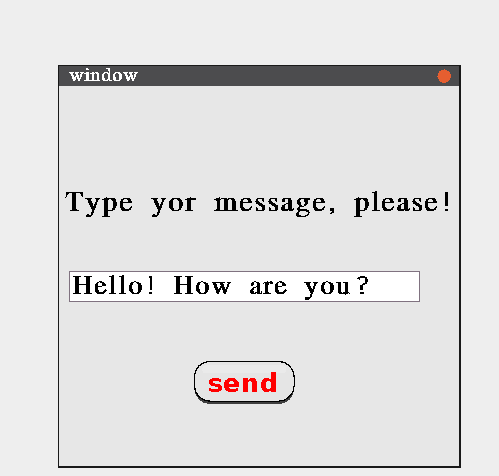
\includegraphics[width=180pt]{pictures/window.png}}
		\caption{ Окно }
		\label{ris:image}
		\end{figure}	
	\pagebreak
	\section{Реализация оконного менеджера}
	\subsection{ Оконная система }
	Перекрытие окон
	inFocus
	draggedElement
	\subsection{ Архитектура оконного менеджера}
	В оконном менеджере будет EventQueue и PrimitiveQueue.
	Eщё он занимается перерисовкой. Он получает вызовает на перерисовку и сам определяет когда перерисовывать. В нем хранится последнее время перерисовки lasttime. Это нужно для того, чтобы слишком часто не перерисовывать экран.
	\pagebreak
	\section{Тестирование и демонстрационный примеры}

	\pagebreak
	
	\section*{Заключение}
	\addcontentsline{toc}{section}{Заключение}
	
	В рамках дипломной работы получены следующие результаты:
	\begin{itemize}
		\item Добавлены примитивы в графическую библиотеку  PostScript.
		\begin{itemize}
			\item Кнопка
			\item Флажок
			\item Поле со списком
			\item Список
			\item Метка
			\item Поле редактирования
			\item Радиокнопка
			\item Окно
		\end{itemize}
		\item Реализован оконный менеджер, интегрированный с графической библиотекой.
		\item Проведено тестирование оконного менеджера на демонстрационных примерах
	\end{itemize}
	

	
	\pagebreak
	\bibliographystyle{ugost2008ls}
	
	
	\begin{thebibliography}{}
		
		\bibitem{PLRM}
		Спецификация языка Postscript. PostScript Language reference. \\
		Adobe Systems. 1999\\
		\url{http://www.adobe.com/products/postscript/pdfs/PLRM.pdf}
		
		\bibitem{jvms}
		Tim Lindholm, Frank Yellin, Gilad Bracha, Alex Buckley.
		The Java Virtual Machine Specification.
		Java SE 7 Edition, 2013. \\
		\url{docs.oracle.com/javase/specs/jvms/se7/jvms7.pdf}
		
		\bibitem{cormen}
		Томас Х. Кормен, Чарльз И. Лейзерсон, Рональд Л. Ривест, Клиффорд Штайн.
		Алгоритмы: построение и анализ.
		Второе издание, 2006
		
	\end{thebibliography}
\end{document}
